\section{Sample Execution}
% Walk through of example query

% Results: figure 1  
\begin{figure}[t]
\centering
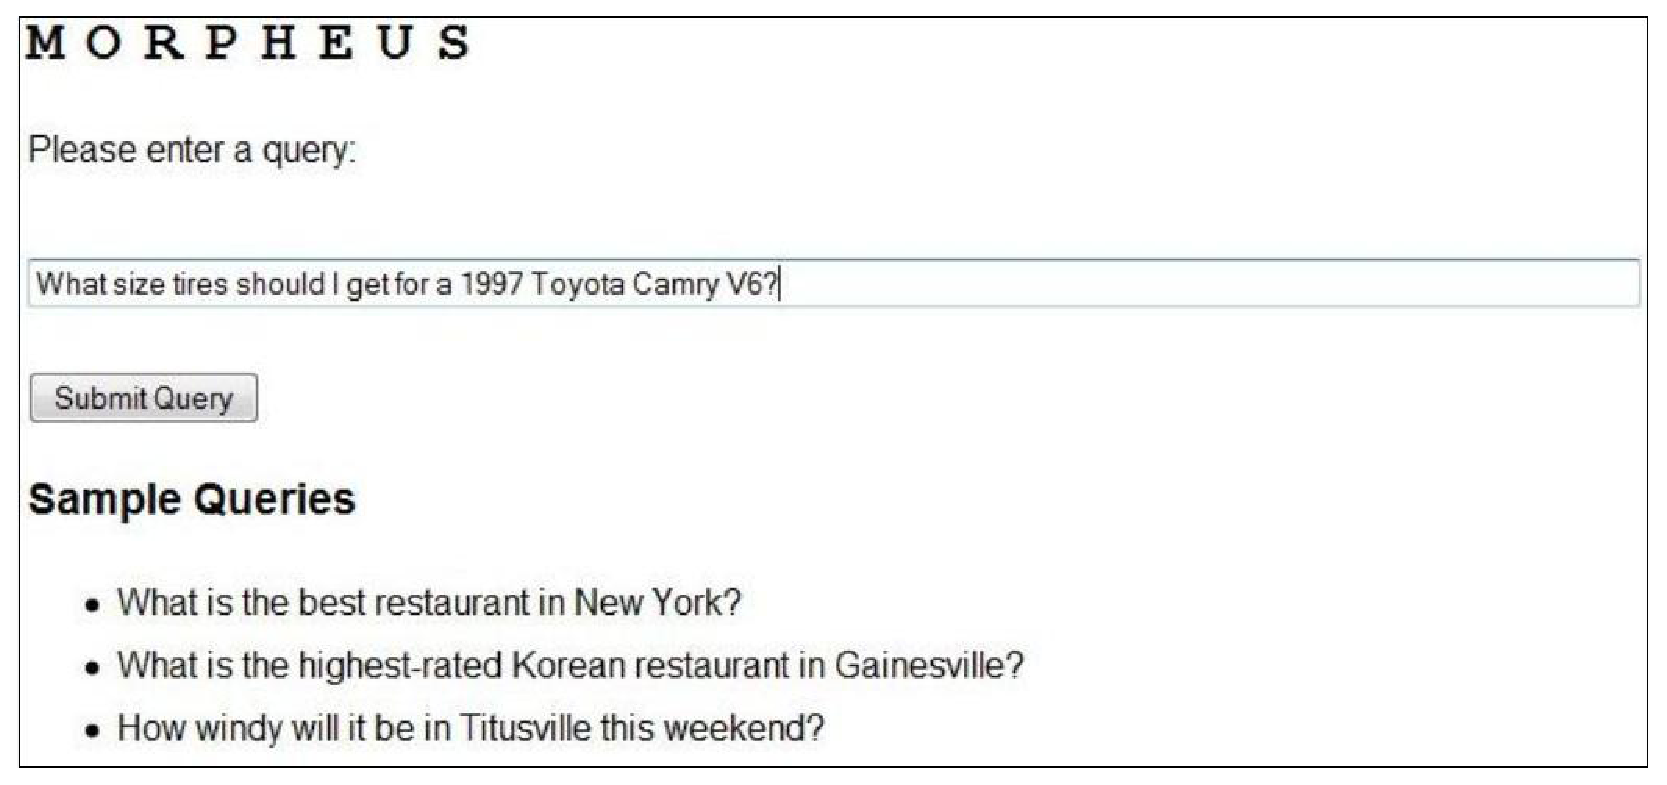
\includegraphics[width=85mm]{screen_intro.eps}
\caption{Morpheus input screen}
\label{fig:screen_intro}
\end{figure}

Figure \ref{fig:screen_intro} shows the Morpheus input screen, which
allows a user to ask a question.  The user enters a natural language
question and the system follows the question answering process outlined
in this document.

% Results: figure 2  
\begin{figure}[t]
\centering
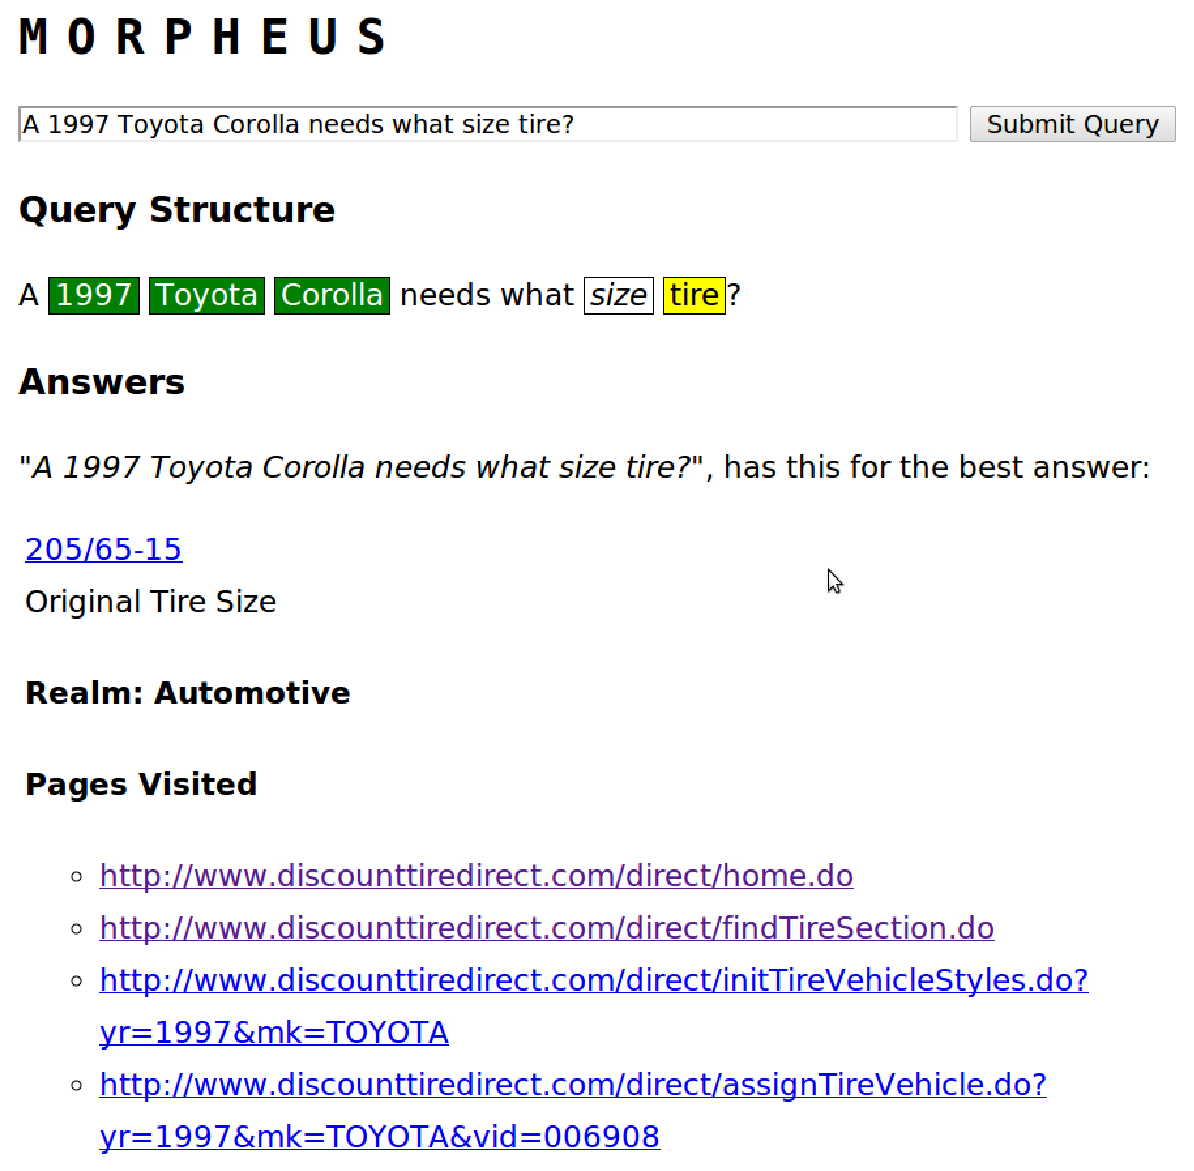
\includegraphics[width=85mm]{screen_result.eps}
\caption{Results screen}
\label{fig:screen_result}
\end{figure}


Figure \ref{fig:screen_result} shows the results of answering the question ``A 1997 Toyota Camry V6 needs what size tire?''
In response to this question, the user is presented with a list of relevant answers and a depiction of how the query was parsed. In the above example, the query about tire size was executed and the most relevant result has been returned and displayed. 
Furthermore, the sequence of pages visited during execution is displayed as well. 

Categories are assigned to the query's SSQ contexts using the method described in section \ref{sec:terms}. The prior probabilities for a variety of categories
together with the likelihood and posterior probabilities for the term \emph{Camry}, e.g. $p(Camry | Automobiles)$ and $p(Automobiles | Camry )$, are as
shown in Table \ref{tab:prob}.
The QRM used to answer this query is selected based on the SSQ matching
process described in section \ref{sec:oqom}.
\begin{table}
  \begin{tabular}{ | l | l | c | r | }
    \hline
    Category & Prior & Likelihood & Posterior \\ \hline
    Automobiles & 0.59 & 3.48e-05 & 0.96 \\ 
    Motorcycles & 0.13 & 2.26e-06 & 0.01 \\
    Internet search engines & 0.16 & 6.29e-07 & 0.004 \\ 
    Lists of countries & 0.06 & 1.50e-06 & 0.01 \\
    Tires & 0.05 & 3.60e-06 & 0.02 \\
    \hline
  \end{tabular}
\caption{Term/Category Probabilities}
\label{tab:prob}
\end{table}

\section{Future Work}

The greatest limitation to our current work is the diversity of the
QRR.  In order to efficiently answer new user questions the systems
needs a large amount of user annotated queries.  However, a
significant number of user interactions is required to understand the
answer retrieval process.  By continuing to study the methods of user
data collection we plan to develop a model to support an unsupervised
question resolution process.  This will increase the scalability and
efficiency of the system.

Because each QRM may be treated as a function, we plan on leveraging
previous work to allow new questions to be solved by connecting
together several QRMs \cite{morpheus1, transformscout}.  This method
would expand the types of queries that are answerable by the system.

Currently, the category heterarchy generated from the DBpedia
categories and our SSQ ontologies is stored in separate XML files. We
are in the process of moving these ontologies into an efficient
ontology database. Similarly, employing user input brings about the
likelihood that redundant SSQ ontological elements will be inserted
into our ontology store. We are working on merging the similar SSQs
[\ref{sec:ssq}] based on the SSQ realms and other ontological
structural information so that we can remove the redundancy in the
database.

We cannot rely on the DBpedia categories and the associated Wikipedia
pages to provide corpora for all our realms.  The DBpedia categories
and the associated Wikipedia documents are insufficient to
characterize the linguistic space of queries belonging to many
different realms.  Reasonable prior probabilities for the names of
musical groups within the category \emph{musical groups}, for example,
will be significantly different from what would be manufactured by
simply finding n-gram frequency within the related Wikipedia
documents. We are investigating methods to identify categories within
the deep web and to find new sources to construct \textit{weak} realms
in our ontology hierarchy.


%% I may have misstated the statistics that are unique/repeats
% need to clarify the statistics 
%% Add language about how we 
Researchers have stated that somewhere from 39 to 63 percent of web
queries are unique \cite{1277770,331405,621942}.  We believe that a
large percentage of the stated unique queries are in-fact related and
parameterizable, meaning, several subsets of unique queries may be all
related and may be answered using a single QRM.  It is difficult to
discover this property between queries.  Previous work suggest
techniques to find related queries but it will take new efficient
methods to discover parameterizable queries.

% Sort classes based on the prior 

\section{Conclusion}

In this paper we provide a discussion on a new type of question
answering system that uses previously answered user questions.  We
described our method of modeling a users question answering process
and how we are able to discover semantically similar queries.  The Morpheus system still has a lot of room for optimization.  However, we believe this new technique for question answering system will improve the exploration experience.


\section{Acknowledgements}
Our thanks to Guillermo Cordero, and Nick Antonelli for thier assistance building this system. Additionally, we would like to thank NSF for their generous support of our project.
